\documentclass[25pt, a1paper,portrait, colspace=5mm, blockverticalspace5mm]{tikzposter}
\tikzposterlatexaffectionproofoff

\usepackage{fontspec}
\usepackage{xcolor}
\usepackage{contour}
\usepackage{pgfplots}
\usepackage{pgfplotstable}
\usepackage{ulem}
\usetikzlibrary{calc, positioning}
\usepackage{graphicx}
\usepackage{booktabs}
\usepackage{ragged2e}
\pagestyle{empty}

\setmainfont{Arial}
\setsansfont{Arial}

\definecolor{CornellRed}{HTML}{B22124}
\definecolor{PosterDark}{HTML}{262626}
\definecolor{BlockGray}{HTML}{F0F0F0}
\definecolor{White}{HTML}{FFFFFF}

\definecolorstyle{wcm}{}{
\colorlet{backgroundcolor}{White} 
\colorlet{framecolor}{White} 
\colorlet{titlebgcolor}{CornellRed} 
\colorlet{titlefgcolor}{White}
\colorlet{titleframecolor}{CornellRed} 
\colorlet{blocktitlebgcolor}{White} \colorlet{blocktitlefgcolor}{black} \colorlet{blockbodybgcolor}{White} 
\colorlet{blockbodyfgcolor}{black}}

\pgfplotstableread{
Model Sens SensLo SensHi Spec SpecLo SpecHi PPV PPVLo PPVHi NPV NPVLo NPVHi Kappa KappaLo KappaHi
Original 0.77 0.14 0.12 0.49 0.08 0.07 0.26 0.08 0.08 0.90 0.06 0.05 0.14 0.08 0.10
Original+Gender 1.00 0.00 0.00 0.04 0.02 0.03 0.20 0.05 0.05 1.00 0.00 0.00 0.02 0.01 0.01
%Adjusted 0.39 0.15 0.16 0.96 0.03 0.03 0.71 0.21 0.18 0.87 0.05 0.05 0.43 0.17 0.15
%Adjusted+Gender 0.40 0.14 0.15 0.96 0.03 0.02 0.71 0.21 0.16 0.87 0.04 0.05 0.43 0.15 0.15
Recalibrated 0.61 0.15 0.14 0.63 0.07 0.07 0.27 0.08 0.10 0.87 0.05 0.06 0.16 0.11 0.12
Recalibrated+Gender 0.68 0.15 0.14 0.65 0.07 0.07 0.31 0.09 0.09 0.90 0.06 0.05 0.22 0.11 0.12
}\datatable

\renewcommand{\ULdepth}{1.8pt}
\contourlength{0.8pt}

\newcommand{\myuline}[1]{%
  \uline{\phantom{#1}}%
  \llap{\contour{white}{#1}}%
}

\usecolorstyle{wcm}
\makeatletter
\definetitlestyle{notrounded}{
    width=\paperwidth,
    roundedcorners=0, % <--- THIS REMOVES THE ROUNDING
}{
    \draw[draw=none, fill=titlebgcolor] 
        (\titleposleft, \titleposbottom) rectangle (\titleposright, \titlepostop);
}
\makeatother

\usetitlestyle{notrounded}

\title{\parbox{\linewidth}{Biological Sex Helps Predict Disposition of Symptomatic \\ Poisoned Patients in the \textbf{ED but not in the ICU}.}}


\begin{document}


\maketitle[titletotopverticalspace=0em, titletoblockverticalspace=0.25cm]

% =====================
% TOP: BACKGROUND
% =====================
\block{\raggedright Predictive Value of Biological Sex for ICU-Level Care}{
\coloredbox[bgcolor=BlockGray, framecolor=White]{
\myuline{\textbf{Background}}
\begin{itemize}
\item Nearly 25\% of poisoned patients admitted to the hospital do not require treatment.
\item The ICU Requirement Score may decrease unnecessary ICU admissions from the ED.
\item Its predictions do not agree with bedside toxicologists.
\item The IRS does not include biological sex, despite its association with poisoning outcomes.
\end{itemize}
\vspace{0.5em}
\textbf{Our goal was to} improve agreement of IRS with toxicologist recommendations by adding biological sex.
}

\vspace{-2.5cm}
}
\note[rotate=20, targetoffsetx=9cm, targetoffsety=4cm]{Try our app,\\ INTOXICALC!
\begin{tikzfigure}

\includegraphics[scale=0.15]{assets/intoxicalc.png}
\end{tikzfigure}
}


% =====================
% MIDDLE: RESULTS
% =====================
\begin{columns}

% ---------- LEFT: FLOW + TABLE ----------
\column{0.5}
\block{}{
\centering
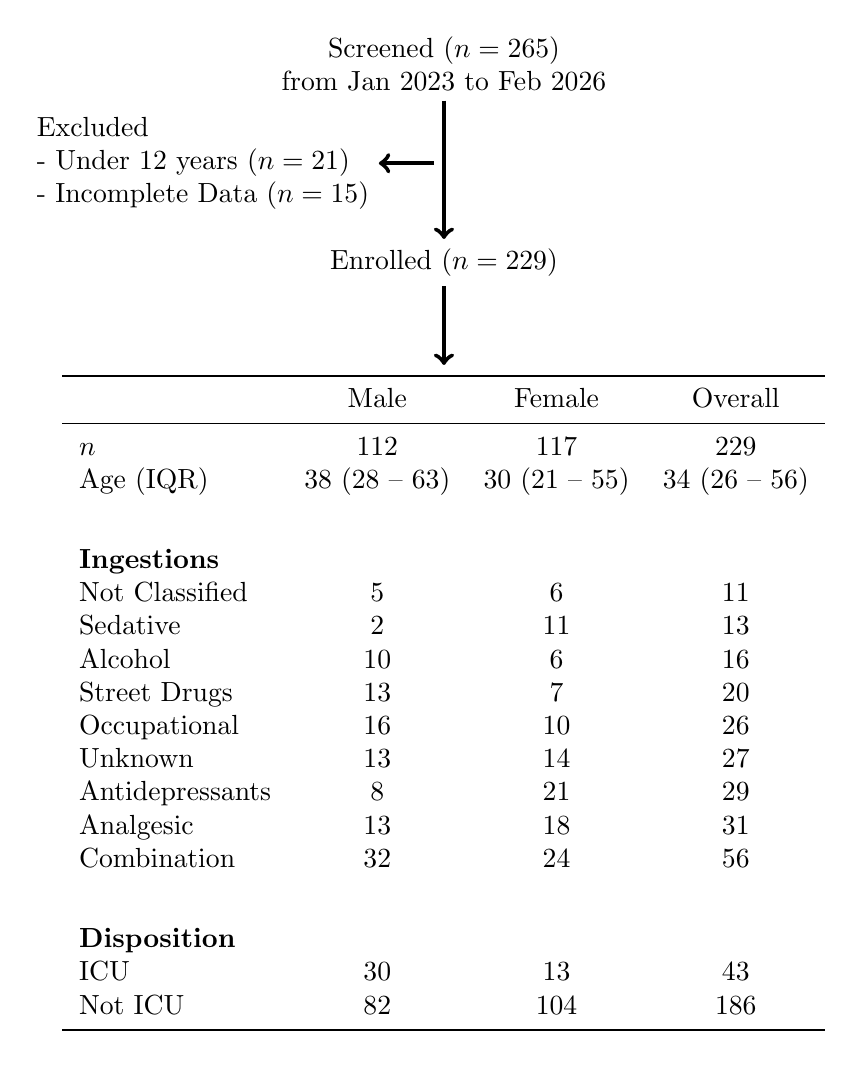
\begin{tikzpicture}

   \node[align=center](screened){Screened $\left(n=265\right)$ \\ from Jan 2023 to Feb 2026};
   \node[below=5em of screened](enrolled){Enrolled $\left(n=229\right)$};
   \node at ($(screened)!0.5!(enrolled)$) (pt){};
   \node[left=2em of pt,align=left](excluded){
       Excluded\\
       - Under $12$ years $\left(n=21\right)$\\
       - Incomplete Data $\left(n=15\right)$};
\node[below=of enrolled](analyzed)
   {   \normalsize
      \begin{tabular}{lccc}
      \toprule
      & Male & Female & Overall \\ \midrule
      $n$ & 112 & 117 & 229 \\
      Age (IQR) & 38 (28 -- 63) & 30 (21 -- 55) & 34 (26 -- 56) \\
      \addlinespace \\
      \textbf{Ingestions} & & & \\ 
      Not Classified & 5 & 6 & 11 \\
      Sedative & 2 & 11 & 13 \\     
      Alcohol & 10 & 6 & 16 \\ 
       Street Drugs & 13 & 7 & 20 \\ 
          Occupational & 16 & 10 & 26 \\
       Unknown & 13 & 14 & 27 \\ 
      Antidepressants & 8 & 21 & 29 \\
      Analgesic & 13 & 18 & 31 \\
      Combination & 32 & 24 & 56 \\  
      
      \addlinespace \\ 
      \textbf{Disposition} & & & \\
      ICU & 30 & 13 & 43 \\ 
      Not ICU  & 82 & 104 & 186 \\\bottomrule
      \end{tabular}
      };

\draw[->, ultra thick] (screened) -- (enrolled);
\draw[->, ultra thick] (pt) -- (excluded);
\draw[->, ultra thick] (enrolled) -- (analyzed);
\end{tikzpicture}
}

% ---------- CENTER: BAR CHART ----------
\column{0.48}
\block{Model Performance}{
\centering
\begin{tikzpicture}
\begin{axis}[
  ybar,
  bar width=25pt,
  width=\linewidth,
  height=0.72\linewidth,
  axis lines*=left,
  ymin=0, ymax=1.05,
  ytick distance=0.25,
  symbolic x coords={
    Original,
    Original+Gender,
    Recalibrated,
    Recalibrated+Gender
  },
  xtick=data,
  xticklabels={Original,+ Sex,ED-Calibrated,+ Sex},
  x tick label style={font=\small},
  ymajorgrids=true,
  grid style={draw=gray!25},
  legend style={at={(0.5,-0.15)}, anchor=north, legend columns=3, draw=none, column sep=1em,
  /tikz/every odd column/.append style={column sep=0.1em}}
]

\addplot+[draw=black, fill=black, error bars/.cd, y dir=both, y explicit]
table[x=Model, y=Sens, y error minus=SensLo, y error plus=SensHi] {\datatable};

\addplot+[draw=black, fill=white, error bars/.cd, y dir=both, y explicit]
table[x=Model, y=Spec, y error minus=SpecLo, y error plus=SpecHi] {\datatable};

\addplot+[draw=CornellRed, fill=CornellRed, error bars/.cd, y dir=both, y explicit]
table[x=Model, y=Kappa, y error minus=KappaLo, y error plus=KappaHi] {\datatable};

\legend{Sensitivity, Specificity, $\kappa$}
\end{axis}
\end{tikzpicture}
}

\block{Agreement with Toxicologists}{
\centering\normalsize

\begin{minipage}{0.5\linewidth}
\centering \textbf{ED-Calibrated Model}

\vspace{0.5em}

\begin{tabular}{lccc}
\toprule
& ICU & Not ICU & Total \\
\midrule
ICU     & 26 & 69  & 95  \\
Not ICU & 17 & 117 & 134 \\
\midrule
Total   & 43 & 186 & 229 \\
\bottomrule
\end{tabular}
\end{minipage}\begin{minipage}{0.5\linewidth}
\centering \textbf{+ Biological Sex} 

\vspace{0.5em}

\begin{tabular}{lccc}
\toprule
& ICU & Not ICU & Total \\
\midrule
ICU     & 29 & 65  & 94  \\
Not ICU & 14 & 121 & 135 \\
\midrule
Total   & 43 & 186 & 229 \\
\bottomrule
\end{tabular}

\end{minipage}
}

\end{columns}
\block{}{
\vspace{-3cm}
\coloredbox[bgcolor=BlockGray, framecolor=White]{
\myuline{\textbf{Methods}}
\begin{itemize} 
\item Secondary analysis of one institutional toxicology registry
\item Refit logistic regression model with and without biological sex.
\item Outcome: Inter-rater agreement between model and toxicologist recommendation
\end{itemize}}

\coloredbox[bgcolor=BlockGray, framecolor=White]{
\myuline{\textbf{Conclusions}:} Including biological sex improves predicting disposition of symptomatic poisoned patients on initial presentation in the ED, but not once in the unit. This may reflect  biological sex functioning as a proxy for dose and ingestion subtype.}

\coloredbox[bgcolor=BlockGray, framecolor=White]{
\myuline{\textbf{Next Steps}}
\begin{itemize} 
\item Including dose | Develop ICU vs Floor vs Home/Psych Model $\Rightarrow$ Prospective Test
\end{itemize}}

\begin{columns}

\coloredbox[bgcolor=CornellRed, framecolor=White, fgcolor=White]{
\begin{minipage}{0.6\textwidth}
Weill Cornell Medicine, Emergency Medicine Research Symposium, 2026 \\
Yash Jaggi, Laibah Ashfaq, Shreya Ranjan, Michael Chary MD, PhD
\end{minipage}\begin{minipage}{0.4\textwidth}
\begin{tikzfigure}

\hspace{-4cm}
\includegraphics[scale=0.7]{assets/logo.png}
\end{tikzfigure}
\end{minipage}
}
\end{columns}
}



\end{document}